\documentclass{article}

\usepackage{fullpage}
\usepackage[doublespacing]{setspace}
\usepackage{amsmath, amssymb,amsfonts}
\usepackage[small]{caption}
\usepackage{graphicx}
\usepackage{float}
\usepackage{subfig}
\usepackage{xspace}
\usepackage{natbib}
\usepackage[normalem]{ulem} %strike out via \sout{}
\usepackage{datetime} %provides \currenttime command
%\usepackage[nomarkers,figuresonly]{endfloat}  %%place all figures at end

\graphicspath{{./Figures/}} \DeclareGraphicsExtensions{.pdf, .jpg, .png}

%BCO: Look at what Science recommends for manuscripts using LaTeX
%(they clearly want to say "go away" but can't):
%http://www.sciencemag.org/site/feature/contribinfo/prep/TeX_help/tex2pdf.xhtml


%%%%%%%%%%%%%%%%%%%%%%%%%%%%%%%%%Local Commands%%%%%%%%%%%%%%%%%%%%%%%%%%%%%
%%% Sort using M-x 'sort-lines'
\newcommand{\Costaobsvec}{\ensuremath{\Cost(\aobsvec)}\xspace}
\newcommand{\Costaveci}{\ensuremath{\Cost(\aveci)}\xspace}
\newcommand{\Costavecj}{\ensuremath{\Cost(\avecj)}\xspace}
\newcommand{\Costavec}{\ensuremath{\Cost(\avec)}\xspace}
\newcommand{\Costcveci}{\ensuremath{\Cost(\cveci)}\xspace}
\newcommand{\Costcvecj}{\ensuremath{\Cost(\cvecj)}\xspace}
\newcommand{\Cost}{\ensuremath{\text{\textbf{C}}}\xspace}
\newcommand{\DeltaAIC}{\ensuremath{\Delta\text{AIC}}\xspace}
\newcommand{\EE}{\mathbb{E}} %use for expectation function E()
\newcommand{\Funcaobsvec}{\ensuremath{\Func(\aobsvec|\aoptvec)}\xspace}
\newcommand{\Funcaoptvec}{\ensuremath{\Func(\aoptvec)}\xspace}
\newcommand{\Funcaveci}{\ensuremath{\Func(\aveci|\aoptvec)}\xspace}
\newcommand{\Funcavecj}{\ensuremath{\Func(\avecj|\aoptvec)}\xspace}
\newcommand{\Funcavec}{\ensuremath{\Func(\avec|\aoptvec)}\xspace}
\newcommand{\Funccveci}{\ensuremath{\Func(\cveci|\aoptvec)}\xspace}
\newcommand{\Funccvec}{\ensuremath{\Func(\cvec|\aoptvec)}\xspace}
\newcommand{\Func}{\ensuremath{\text{\textbf{B}}}\xspace}
\newcommand{\GTR}{GTR+$\Gamma$\xspace}
\newcommand{\LogN}{\ensuremath{\text{LogN}}\xspace}
\newcommand{\Ne}{\ensuremath{{N_e}}\xspace} %
\newcommand{\Nemu}{\ensuremath{{N_e \mu}}\xspace} %
\newcommand{\Lik}{\ensuremath{\mathcal{L}}\xspace}%replaces \Lmatrix which was inconsistent and, thus, confusing 
\newcommand{\pimatrix}{\ensuremath{\mathbf{\pi}}\xspace}
\newcommand{\mumatrix}{\ensuremath{\mathbf{\mu}}\xspace}
\newcommand{\Pmatrix}{\ensuremath{\mathbf{P}}\xspace}
\newcommand{\Tmatrix}{\ensuremath{\mathbf{T}}\xspace}
\newcommand{\Dmatrix}{\ensuremath{\mathbf{D}}\xspace}
\newcommand{\Dmatrixp}{\ensuremath{\mathbf{D}_p}\xspace}
\newcommand{\Mmatrix}{\ensuremath{\mathbf{M}}\xspace}
\newcommand{\Qmatrix}{\ensuremath{\mathbf{Q}}\xspace}
\newcommand{\Qmatrixa}{\ensuremath{\Qmatrix_a}\xspace}
\newcommand{\Wi}{\ensuremath{{W_i}}\xspace}
\newcommand{\Wj}{\ensuremath{{W_j}}\xspace}
\newcommand{\simP}{\ensuremath{\sim P}\xspace}
\newcommand{\acivec}{\ensuremath{a\left(\cveci\right)}\xspace}
\newcommand{\acvecg}{\ensuremath{a\left(\vec{c}_{i,g}\right)}\xspace}
\newcommand{\acvecj}{\ensuremath{a\left(\cvecj\right)}\xspace}
\newcommand{\acvec}{\ensuremath{a\left(\Vec{c}\right)}\xspace}
\newcommand{\aip}{\ensuremath{a_{i,p}}\xspace}
\newcommand{\aivecg}{\ensuremath{{\avec}_{i,g}}\xspace}
\newcommand{\aivec}{\aveci}
\newcommand{\ajp}{\ensuremath{a_{j,p}}\xspace}
\newcommand{\ajvecg}{\ensuremath{{\ajvec}_{,g}}\xspace}
\newcommand{\ajvec}{\ensuremath{\Vec{a}_{j}}\xspace}
\newcommand{\aj}{\ensuremath{a__j}\xspace}
\newcommand{\alphac}{\ensuremath{\alpha_c}\xspace}
\newcommand{\alphag}{\ensuremath{\alpha_G}\xspace}
\newcommand{\alphap}{\ensuremath{\alpha_p}\xspace}
\newcommand{\alphavec}{\ensuremath{\Vec{\alpha}}\xspace}
\newcommand{\alphav}{\ensuremath{\alpha_v}\xspace}
\newcommand{\alphavValue}{\ensuremath{4 \times 10^{-4}}\xspace}
\newcommand{\aobsvecg}{\ensuremath{{\avec}_{\text{obs},g}}\xspace}
\newcommand{\aobsvec}{\ensuremath{\Vec{a}_{\text{obs}}}\xspace}
\newcommand{\aobs}{\ensuremath{a_{\text{obs}}}\xspace}
\newcommand{\aopt}{\ensuremath{a_*}\xspace}
\newcommand{\aoptip}{\ensuremath{\aopt_{i,p}}\xspace}
\newcommand{\aoptpg}{\ensuremath{\aopt_{p,g}}\xspace}
\newcommand{\aoptp}{\ensuremath{a_{*,p}}\xspace}
\newcommand{\aoptvecg}{\ensuremath{{{\aoptvec}_g}}\xspace}
\newcommand{\aoptvec}{\ensuremath{\Vec{a}_*}\xspace}
\newcommand{\aveci}{\ensuremath{\Vec{a}_i}\xspace}
\newcommand{\avecj}{\ensuremath{\Vec{a}_j}\xspace}
\newcommand{\avec}{\ensuremath{\Vec{a}}\xspace}
\newcommand{\cveci}{\ensuremath{\cvec_i}\xspace}
\newcommand{\cvecj}{\ensuremath{\cvec_j}\xspace}
\newcommand{\cvec}{\ensuremath{\Vec{c}}\xspace}
\newcommand{\deltaT}{\ensuremath{\delta t}\xspace}
\newcommand{\etag}{\ensuremath{\eta_g}\xspace}
\newcommand{\fij}{\ensuremath{f_{i,j}}\xspace}
\newcommand{\jmax}{\ensuremath{{j_{\max}}}\xspace}
\newcommand{\kmax}{\ensuremath{{k_{\max}}}\xspace}
\newcommand{\muij}{\ensuremath{\mu_{i,j}}\xspace}
\newcommand{\muvec}{\ensuremath{\Vec{\mu}}\xspace}
\newcommand{\phig}{\ensuremath{\phi_{g}}\xspace}
\newcommand{\psig}{\ensuremath{\psi_{g}}\xspace}
\newcommand{\psiprime}{\ensuremath{\psi^\prime}\xspace}
\newcommand{\pij}{\ensuremath{p_{i,j}}\xspace}
\newcommand{\qij}{\ensuremath{q_{i,j}}\xspace}
\newcommand{\qji}{\ensuremath{q_{i,j}}\xspace}
\newcommand{\setG}{\ensuremath{\mathbb{G}}\xspace}
\newcommand{\setP}{\ensuremath{\mathbb{P}}\xspace}
\renewcommand{\ng}{\ensuremath{{n_g}}\xspace}
\newcommand{\gp}{\ensuremath{{G_p}}\xspace}
\DeclareMathOperator{\Var}{Var}

\title{Population Genetics Based Phylogenetics Under Stabilizing Selection for an Optimal Amino Acid Sequence: A Nested Modeling Approach
} \date{Last compiled on \today\xspace at \currenttime.}
\begin{document}
\maketitle


\section*{Abstract}
We present a phylogenetic approach rooted in the field of population genetics that more realistically models the evolution of protein-coding DNA under the assumption of stabilizing selection for a gene specific optimal amino acid sequence.
The new set of models, which we collectively call selac models, fit phylogenetic data substantially better than popular current models, suggesting more accurate inference of phylogenetic trees and branch lengths.
Moreover, these models allow inference of population genetics parameters from data used for interspecific phylogenies.

\section*{Introduction}
Phylogenetic analysis now plays a critical role in the fields of ecology, evolution, paleontology, medicine, conservation, and many others.
While the scale and impact of phylogenetic studies has increased substantially over the past two decades, by comparison the realism of the mathematical models on which these analyses are based has changed relatively little.
The simplest but most popular models are agnostic with regards to the different amino acid substitutions and may or may not include mutation bias (e.g.~F81, F84, HYK85, TN93, and GTR for the former and JC69 and K80 for the latter, see \citet{Yang2014} for an overview).

Another set of models attempt to include a 'selection' term $\omega$, however the link between $\omega$ and the key parameters found in standard population genetics models such as \Ne, the distribution of fitness across genotype space, and mutation bias are far from clear.
For instance, $\omega$ is generally interpreted as indicating whether a sequence is under `purifying' ($\omega < 1$) or `diversifying' ($\omega > 1$) selection.
However, the actual behavior of the model as is quite different.
When $\omega < 1$ the model behaves as if the resident amino acid $i$ at a given site is favored by selection since synonymous substitutions have a higher substitution rate than any possible non-synonymous substitutions.
Paradoxically, this selection regime for the resident amino acid $i$ persists \emph{until} a substitution for another amino acid, $j$, occurs.
As soon as amino acid $j$ fixes, but not before, selection now favors amino acid $j$ over all other amino acids, including $i$.
This is now the opposite scenario to when $i$ was the resident.
Similarly, when $\omega > 1$, synonymous substitutions have a lower substitution rate than any possible non-synonymous substitutions the resident amino acid.
In a parallel manner, this selection \emph{against} on the resident amino acid $i$ persists until a substitution occurs at which point selection now \emph{favors}  the former resident amino acid $i$ as well as the 18 others.
Thus, the simplest and most consistent interpretation of $\omega$ is that it describes the rate at which the selection regime itself changes, and this change in selection perfectly coincides with the fixation of a new amino acid.
As a result, $\omega$ based approaches likely only describe a subset of scenarios such as over/underdominance or frequency dependent selection \citep{HughesAndNei1988,Nowak2006}.

Fortunately, given the continual growth in computational power available to researchers, it is now possible to utilize a more general set of population genetics based models for the purpose of phylogenetic analysis \citep[e.g.][]{HalpernAndBruno1998,RobinsonEtAl2003,LartillotAndPhilippe2004,RodrigueAndLartillot2014}.
One lesson from the field of population genetics is while there are only a few fundamental evolutionary forces at play (mutation, drift, selection, and linkage effects) describing the evolutionary behavior of a system in which there are non-linear interactions between different sites quickly becomes extremely challenging.
Fortunately, under the simplifying assumptions of additivity between sites and alleles, calculating stationary and substitution probabilities are relatively straightforward, making fitting additive models of the evolutionary process to sequence data computationally feasible.

Another major advantage to our approach is that the parameters estimated are biologically meaningful.
As with other phylogenetic methods,  we generate estimates of branch lengths and nucleotide specific mutation rates.
In addition, because the math behind our model is mechanistically derived, our method can also be used to make quantitative inferences on the optimal amino acid sequence of a given protein as well as the average synthesis rate of each protein used in the analysis.
The mechanistic basis of our model also means it can be easily extended to include more biological realism and test more explicit hypotheses about sequence evolution.

We model the substitution process as a classic Wright-Fisher process which includes the forces of mutation, selection, and drift \citep{Fisher1930,Kimura1962,Wright1969,Iwasa1988,BergAndLassig2003,SellaAndHirsh2005,McCandlishAndStoltzfus2014}.
For simplicity, we ignore linkage effects and, as a result of this and other assumptions, our model behaves in a site independent manner.
Our approach is developed in the same vein as previous phylogenetic applications of the Wright-Fisher process \citep[e.g.][]{MuseAndGaut1994,HalpernAndBruno1998,YangAndNielsen2008,RodrigueEtAl2005,KoshiAndGoldstein1997,KoshiEtAl1999,DimmicEtAl2000,ThorneEtAl2012,LartillotAndPhilippe2004,RodrigueAndLartillot2014}.
Similar to Lartillot's work \citep{LartillotAndPhilippe2004,RodrigueAndLartillot2014}, we assume there is a finite set of rate matrices describing the substitution process and that each position within a protein must assigned to a particular rate matrix category.
Unlike these other researchers, we assume \emph{a priori} there are 20 different families of rate matrices, one family for when a given amino acid is favored at a site.
As a result, our approach allows us to quantitatively evaluate the support for a particular amino acid being favored at a particular position within the protein encoded by a particular gene.

Because our approach requires twenty families of $61 \times 61$ matrices, the number of parameters needed to implement our model would, without further simplification, be extremely large.
To reduce the number of parameters needed while still maintaining a high degree of biological realism, we construct our gene and amino acid specific substitution matrices using a submodel nested within our substitution model.
We've utilized the same nested, population genetic based approach in more traditional genomic analyses \citep[e.g.][]{Gilchrist2007,ShahAndGilchrist2011,GilchristEtAl2015}.
That work and our current work illustrates how more information can be extracted from sequence data when more biologically based models are used.

One advantage of a nested modeling framework is that it requires only a handful of genome wide parameters such as nucleotide specific mutation rates (scaled by effective population size \Ne), side chain physiochemical weighting parameters, and a shape parameter describing the distribution of site sensitivities. % around a mean value of 1.
In addition to these genome wide parameters, our model requires a gene $g$ specific expression parameter $\psi_g$ which describes the average rate at which the protein's functionality is produced by the organism.
The gene specific parameter $\psi_g$ is multiplied by additional model terms to make a composite term $\psiprime_g$ which scales the strength and efficacy of selection for the optimal amino acid sequence.\footnote{should we introduce the \aopt notation here?}
Our model also requires the designation of an optimal amino acid at each position or site within a coding sequence which, in turn, makes it the largest category of parameters we estimate.
Because we use a submodel to derive our substitution matrices, our model requires the estimation of a fraction of the parameters required when compared to approaches where the substitution rates are allowed to vary independently \citep{HalpernAndBruno1998,LartillotAndPhilippe2004,RodrigueAndLartillot2014}.
This, in turn, allows us to move beyond simply generating MLE estimates of parameters \citep[c.f.][]{YangAndNielsen2008} and quantify our uncertainty in these values.

The work we present here contributes to the field of phylogenetics and molecular evolution in a number of ways.
Our model provides an complementary example to \citet{ThorneEtAl2012} studies of how models of molecular and evolutionary scales can be combined together in a nested manner.
While the mapping between genotype and phenotype is more abstract than \citet{ThorneEtAl2012}, our approach has the advantage of not requiring knowledge of a protein's native folding.
Our use of model nesting also allows us to formulate and test specific biological hypotheses.
For example, we are able to compare a model formulation which assumes that physio-chemical deviations from the optimal sequence are equally disruptive at all sites within a protein to one which assumes the effect of deviation from the optimal amino acid's physiochemical properties on protein function varies between sites.
By linking the strength of stabilizing selection for an optimal amino acid sequence to gene expression,  we can weight the historical information encoded in genes evolving at vastly different rates in a biologically plausible manner while simultaneously estimating their expression levels.
Finally, because our work fitness functions are well defined, we can provide estimates of key evolutionary statistics such as the distribution of effects on fitness and genetic load.



\section*{Results}
By linking transition rates $\qij$ to gene expression $\psi$, our approach allows use the same model for genes under varying degrees of purifying selection.
Specifically, we assume the strength of stabilizing selection for the optimal sequence, \aoptvec, is proportional to $\psi$, our model allows us to estimate $\phi = \psi/\Func$ for each gene. 
Our results clearly indicate that accounting for it substantially improves our model fit.
Using both \DeltaAIC and \AICw as our measure of model support, the SelAC models perform extraordinarily better than GTR+$\Gamma$, GY94, or YN08.
This improvement is in spite of the need for estimating the optimal amino acid at each position in each protein, which adds more than 47,000 more parameters to the model than YN08, the next most parameter rich codon model in our model set.
Nevertheless, the SelAC model shows nearly 400,000 AIC unit improvement over YN08.
Comparing the two SelAC models in the model set, including the random effects term $\alphag$ not only provides greater biological realism by allowing site heterogeneity, it also provides substantially better model fit and improves the \DeltaAIC score by over 23,000 units than assuming $\alphag = \infty$. 

With respect to estimates of $\psi$ within SelAC, they were strongly correlated with two separate empirical measurements taken during log growth phase (See Figure). In other words, using only codon sequences our model can predict which genes have high or low expression levels.
The estimate of the $\alphag$ parameter, which describes the site-specific variation in sensitivity of the proteins functionality, indicated a moderate level of variation in gene expression among sites.
Our estimate of $\alphag$ = 1.40, produced a distribution of sensitivity rates that ranged from 0.344 - 7.16, but with the nearly 90\% of the weight for a given site-likelihood being contributed by the 0.344 and 1.48 rate categories.
In simulation, however, of all the parameters in the model, only $\alphag$ showed a consistent bias, in that the estimates were generally underestimated (see Supplemental). Other parameters in the model, such as the Grantham weights, provide an indication as to the physiochemical distance between amino acids.
Our estimates of these weights only strongly deviate from Grantham's composition weight, $\alphac$, which is the distance between any two amino acids with regards to the ratio of noncarbon elements in the end groups to the number of side chains.
We estimate the weighting factor of composition to be $\alphac$=0.484, which suggests that the reduction in the distance between any given two amino acids and greater exchangeability between even the most distantly related residues.

It is important to note that the nonsynonymous/synonymous mutation ratio, or $\omega$, which we estimated for each gene under the FMutSel0 model strongly correlated with our estimates of $\psi$.
In fact, the $\omega$ showed similar, though slightly reduced correlations, with our empirical estimates of gene expression (See Figure).
This would give the impression that the same conclusions could have been gleaned using a much simpler model, both in terms of the number of parameters and the assumptions made.
However, when we evaluated each model by the realistic nature of the data they produce, our SelAC model clearly performs better.
When we simulated the sequence for \textit{S. cervisieae}, starting from the ancestral sequence under both GTR+G and FMutSel0, the functionality of the simulated sequence moves away from the observed sequence, whereas SelAC remains near the functionality of the observed sequence (Figure XX).
In a way, this is somewhat unsurprising, given that both GTR+G and FMutSel0 are agnostic with regards to the functionality of the gene, but it does highlight the improvement in biological realism in codon evolution that our SelAC provides.
We do note that the adequacy of the SelAC model does vary among individual taxa, and does not always perfectly match the observed functionality.
For instance, \textit{S. castellii} is simulated with consistently higher functionality than observed (Figure XX).
We suspect this is an indication that assuming a single set of optimal amino acid across all taxa may be too simplistic, though, at the moment, we cannot also rule out other potential issues in our model, such as a single set of Grantham weights and $\alphag$.


\subsection*{Figures}
\begin{enumerate}
\item Branch Lengths
\newcommand{\subfigwidth}{0.4\textwidth}
\begin{figure}[H]
  \centering
  \subfloat[\ ]{\frame{\includegraphics[width=\subfigwidth]{yeast_SELACgamma.pdf}}}
  \qquad
  \subfloat[\ ]{\frame{\includegraphics[width=\subfigwidth]{yeast_SELACnogamma.pdf}}}
  \qquad
  \subfloat[\ ]{\frame{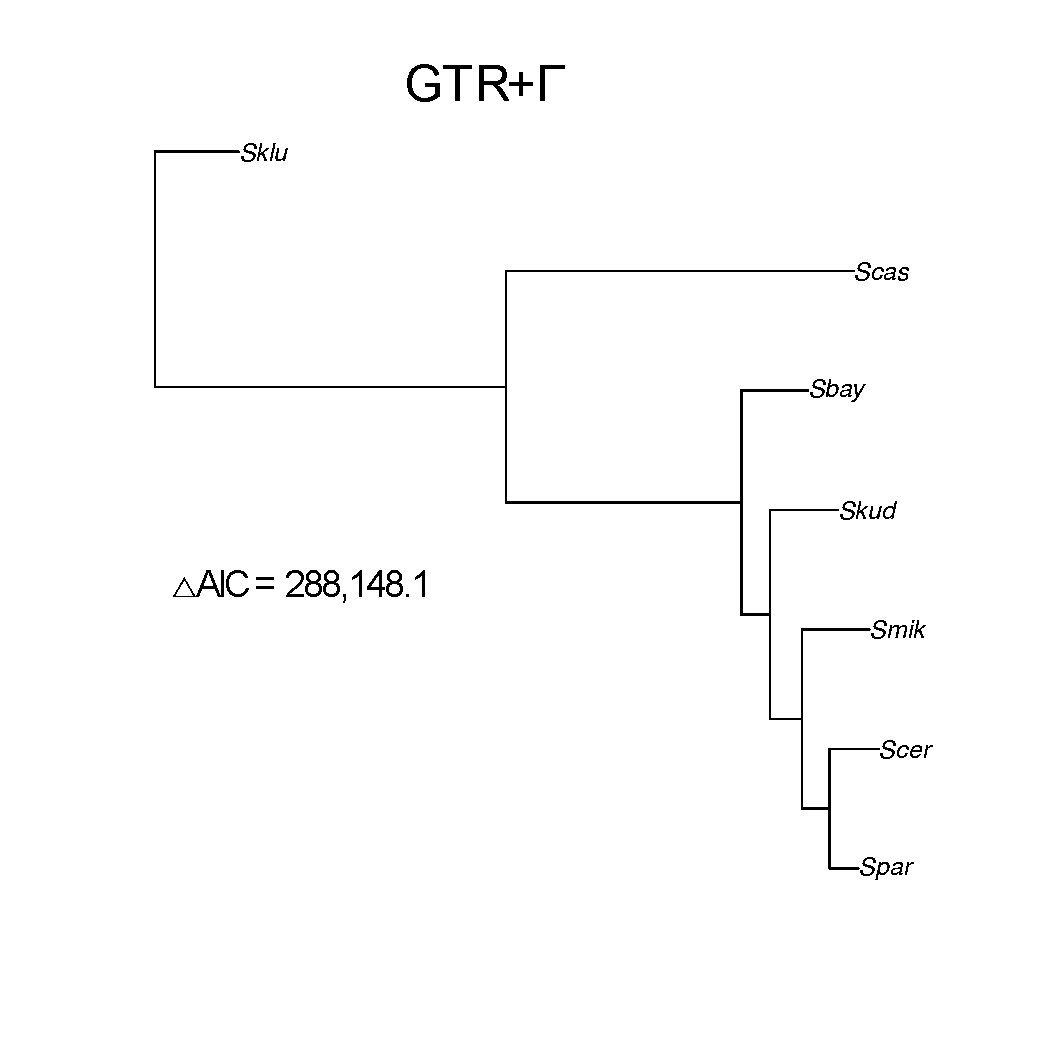
\includegraphics[width=\subfigwidth]{yeast_GTR.pdf}}}
  \qquad
  \subfloat[\ ]{\frame{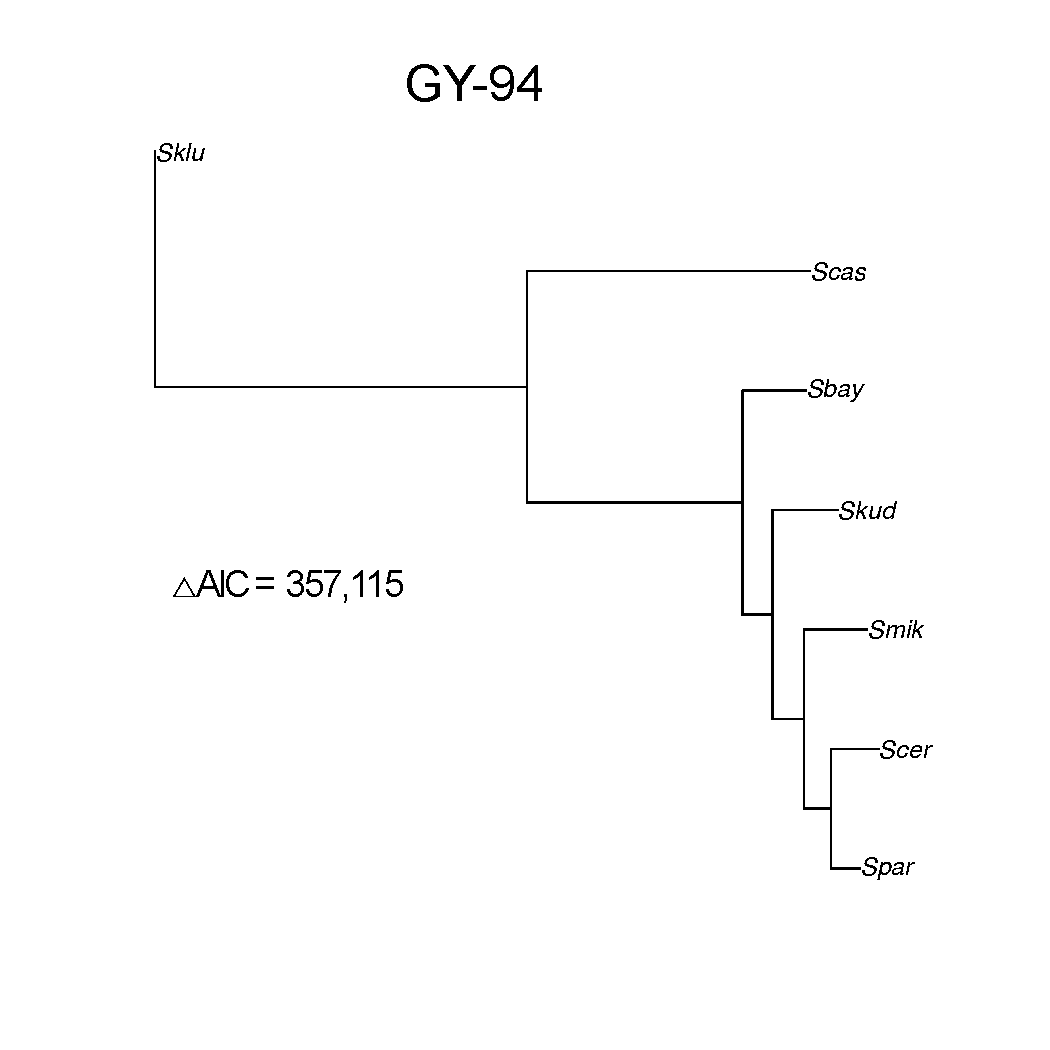
\includegraphics[width=\subfigwidth]{yeast_GY94.pdf}}}
  \qquad
  \subfloat[\ ]{\frame{\includegraphics[width=\subfigwidth]{yeast_YN2008.pdf}}}
  \qquad
  \subfloat[\ ]{\frame{\includegraphics[width=\subfigwidth]{yeast_LGY2004.pdf}}}\footnote{File 'yeast\_LGY2005.pdf' missing from /Figures}
  \caption{Maximum Likelihood Trees for (a) selac, (b) selac with uniform sensitivity $G = 1$, (c) GTR, (d) GY94, and (e) YN08, (f) \citet{LartillotAndPhilippe2004}.}
  \label{fig:mleTrees}
\end{figure}
\item Model Adequacy Illustrations \label{fig:modelAdequacy} (Brian or Jeremy?)
\item Gene Expression Comparisons \label{fig:phiComparisons} (Mike, trying to get data for additional yeast species.)
  \renewcommand{\subfigwidth}{0.4\textwidth}
  \begin{enumerate}
  \item SelAC vs. Empirical  Measurements
    \begin{figure}[H]
      \centering
      \subfloat[\ ]{\frame{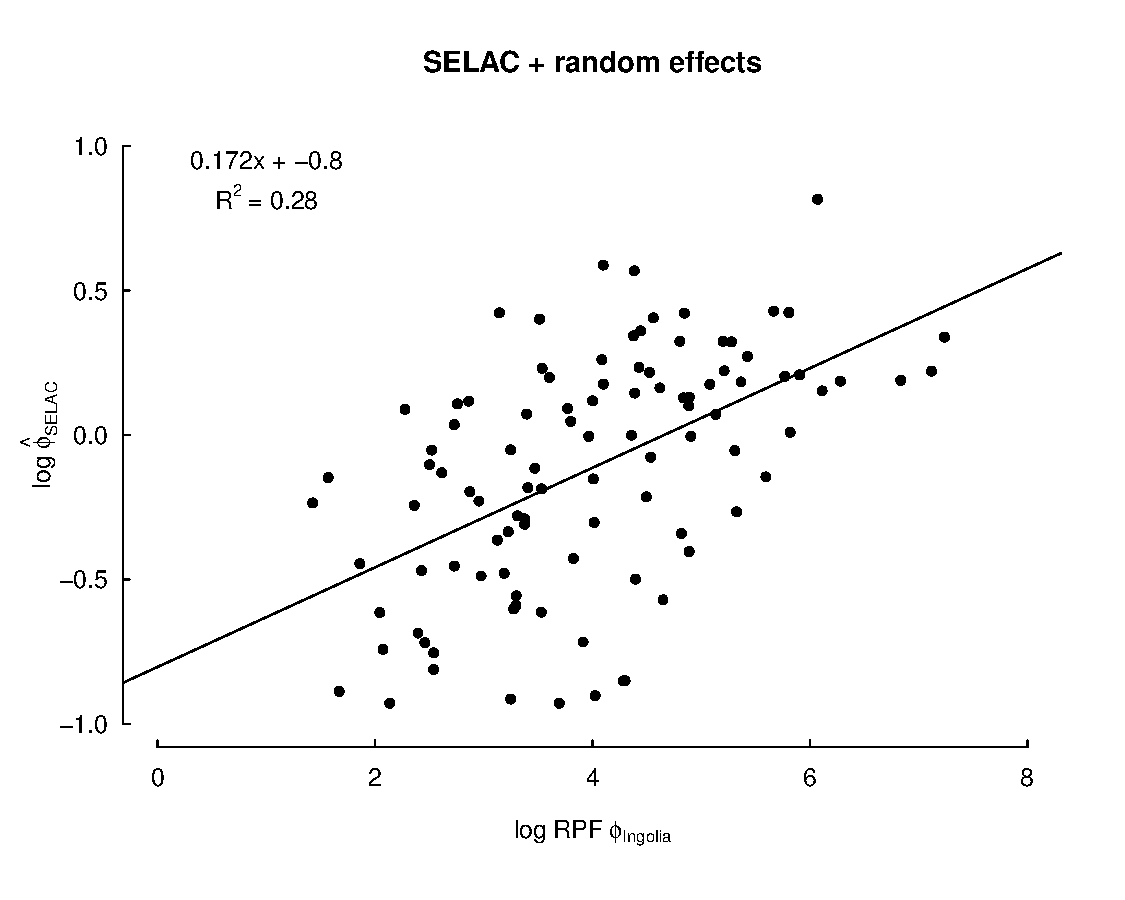
\includegraphics[width=\subfigwidth]{RPF_vs_Phi/RNA_abunIngolia_vs_SelACphiGamma}}}
      \qquad
      \subfloat[\ ]{\frame{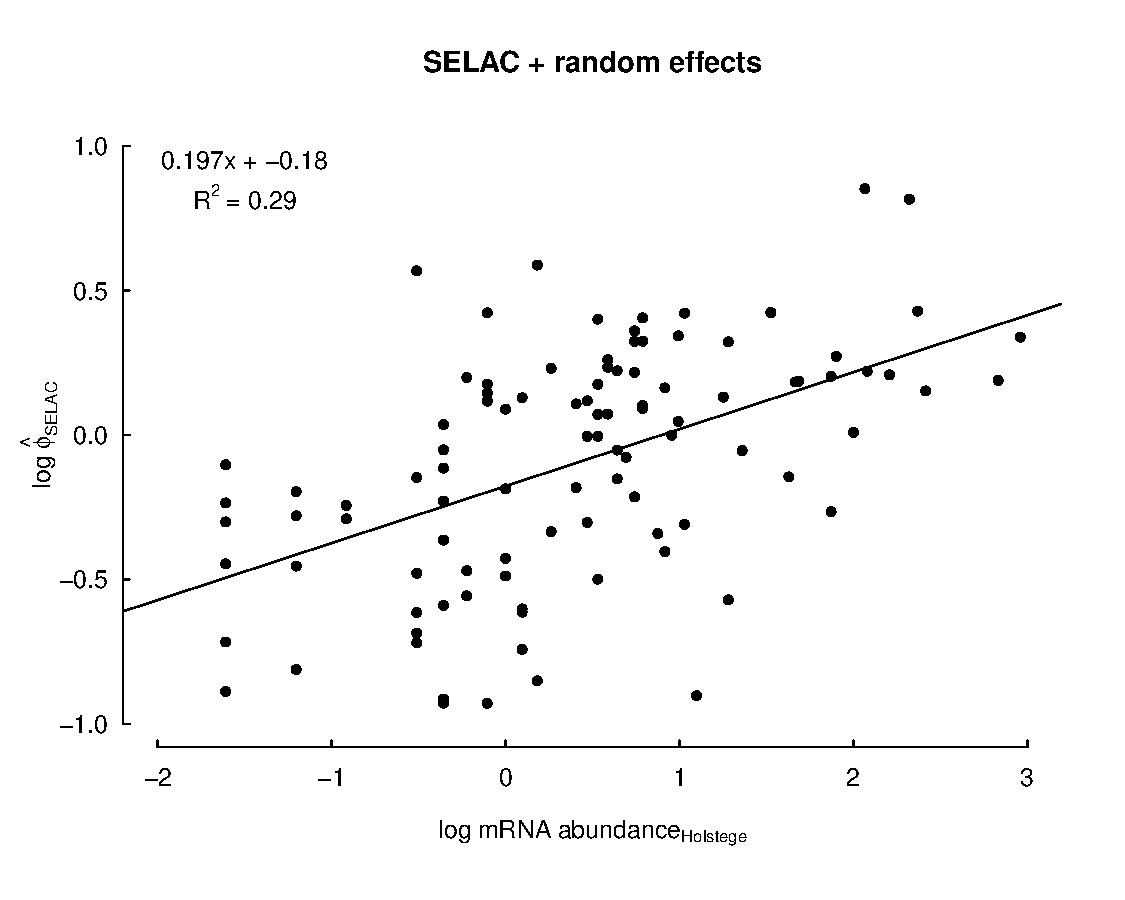
\includegraphics[width=\subfigwidth]{mRNA_vs_Phi/mRNA_abunHolstege_vs_SelACphiGamma}}}
      \caption{Comparison of log protein synthesis rate $\psi$ for \emph{S.~cerevisiae} as predicted by selac to empirical estimates from (a) ribosome profile footprint data \citep{IngoliaEtAl2009} and (b) mRNA abundance data \citep{HolstegeEtAl1998}.
      }
    \end{figure}
  \item SelAC vs.~ROC Measurements (should probably go in Supporting Materials)
    \begin{figure}[H]
      \centering
      \includegraphics[width=0.9\linewidth]{phi_roc_vs_selac-nup.pdf}
    \end{figure}
  \end{enumerate}
\item Quantifying optimal AA \label{fig:optAA} (Mike once I get info from Jeremy)
  \begin{enumerate}
  \item Represent using varying point size in 3D physiochemical space
  \item Look for instances where there's a bimodal distribution across.
    This would suggest a shift in optimal AA.
  \end{enumerate}
\item Visualization of Evolutionary Landscapes (Brian)
  \begin{enumerate}
  \item Summary of Fitness Landscapes: frequency distribution of $W_i$ with varying $\psi$. \label{fig:fitnessLandscape}
  \item Stationary Distribution of Fitness Values: Frequency distribution of $\exp[W_i]$ with varying $\psi$. \label{fig:expectedGeneticLoad}
    Essentially above figure, but $W_i$ values are evaluated based on their stationary probability distribution.
    These figures can be related to concepts about genetic load.
  \item Distribution of Mutation Fitness Effects: Frequency distribution at which new mutants with fitness value $\exp[W_m]$ are introduced at stationarity. \label{fig:mutationFitnessEffects}
  \end{enumerate}
\end{enumerate}


\subsection*{Tables}
\begin{enumerate}
\item Model Fit Summary:
  Table of number of parameters,
  estimates for key parameters (or their summaries), and \DeltaAIC
  values.
  \begin{table}
    \begin{tabular}{lrrrrl}
      &          &Parameters &          &        & Model\\
      Model                 	& logLik   & Estimated &     AIC& \DeltaAIC&  Weight\\\hline
      GTR+$\Gamma$        		& -655166.4&        610& 1,311,553& 504,151&$<$0.001\\
      GY94                  	& -612121.5&        210& 1,224,663& 417,261&$<$0.001\\
      YN08              		& -598848.2&       2810& 1,203,316& 395,914&$<$0.001\\
      SelAC: UNREST         	& -465616.7&       50,004&   831,226&  23,824&$<$0.001\\
      SelAC: UNREST+$\Gamma$ 	& -453706.0&       50,005&   807,402&       0& 0.999
    \end{tabular}
    \caption{Model comparisons}\label{table:modelFits}
  \end{table}
\end{enumerate}
\section*{Discussion}
As phylogenetic methods become ever more ubiquitous in biology, and data set size and complexity increase, there is a need and an opportunity for more complex and realistic models \citep{GoldmanEtAl1996,ThorneEtAl1996,GoldmanEtAl1998,HalpernAndBruno1998,LartillotAndPhilippe2004} %citations identified in Lartillot and Philippe 2004
  \footnote{mikeg: Jeremy and Brian, can you provide some references that make this statement but only make minor advances? JMB -- not sure I understand this. Yes, we have many different matrices, but that's only out of coding convenience. It is actually a single 1344x1344 matrix. If you are thinking about the fact we multiply the mutation matrix by the fixation matrix, you can actually generate two matrices for MutSel and multiply them together (see pg 570 of that paper.)
mikeg: I mean, single 20x20 or 64x64 matrix used for all sites.
So GY2008 would not fall into this definition.: JMB: Ok. And I forgot that even though the off-diagonals are technically zero, the diagonals are not exponeniated with respect to the big matrix, only individually, so it is multiple matrices, not a single model.}.
Despite their widespread use, phylogenetic models based on purifying and diversifying selection,i.e.~\citet{GoldmanAndYang1994} and its extensions, are very narrow categories of selection that mostly apply to cases of positive and negative frequency dependent selection at the level of a particular amino acid.

Instead of heuristically extending population genetic models of neutral evolution for use in phylogenetics, it makes sense to derive these extensions from population genetic models that \emph{explicitly} include the fundamental forces of mutation, drift, and natural selection. % (i.e.~a Wright-Fisher model).
Starting with \citet{HalpernAndBruno1998}, a number of researchers have developed methods for linking site specific selection on protein sequence and phylogenetics\citep[e.g.~][]{KoshiEtAl1999,DimmicEtAl2000,KoshiAndGoldstein2001,RobinsonEtAl2003,LartillotAndPhilippe2004,ThorneEtAl2012,RodrigueAndLartillot2014}.%[CHECK CITATIONS].
Our work follows this tradition, but includes some key advances.
For example, even though our model requires a large number of matrices, because of our assumption about protein functionality and physiochemical distance from the optimum, we are able to parameterize our substitution matrices using a relatively small number of genome wide parameters and one gene specific parameter.
We show that all of these parameters can be estimated simultaneously with branch lengths from the data at the tips of the tree.
By assuming fitness declines with extraneous energy flux, our model explicitly links the variation in the strength of stabilizing selection for the optimal protein sequence between genes to the variation in the target expression level $\psi$.
In turn, our model allows us to generate quantiative estimates of gene expression and amino acid optimality (Figures \ref{fig:phiComparisons} and \ref{fig:optAA}) and link molecular evolution and function.
Our results indicate that including a gene specific $\psi$ value vastly improves our model fits (Table \ref{table:modelFits} and Figure \ref{fig:phiComparisons})).
Of course, given the general nature of our model and the complexity of biological systems, other biological forces also contribute to gene level variation in natural selection.
Nevertheless, the idea that the strength of stabilizing selection and gene expression are positively correlated is well supported by other researchers \citep[e.g.][]{DrummondEtAl2005} and we find that the target expression level $\psi$ and realized protein synthesis rate $\phi$ are reasonably well correlated with laboratory measurements of gene expression.

Additional advantages
\begin{enumerate}
\item More realistic behavior over time: Model adequacy (Figure \ref{fig:modelAdequacy} )
\item Improved fit (Table \ref{table:modelFits})
\item Improved estimates of branch lengths and mutation: A better model gives you a better answer \ref{fig:mleTrees}
\item Better biological interpretation and more biological information.
\item Likelihood based estimate ancestor state rather consensus assumption.
\item Approach can even be expanded to other types of sequence data in which selection can be reasonably modeled, e.g.~UCEs.
\item Allows us to describe evolutionary process using our inferred fitness landscapes (Figures \ref{fig:fitnessLandscape}-\ref{fig:mutationFitnessEffects}.
\end{enumerate}


The fact that our approach allows us to estimate gene expression from phylogenetic data has a number of important implications by itself.
\begin{itemize}
\item First, it indicates there is substantially more information in the coding sequences used for phylogenetic analysis than other methods acknowledge.
\item Second, it demonstrates how selection can be modeled as the product of two separate components.
  Here we use gene expression $\psi$ and protein function \Func, but more complex models could clearly be used.  Finally, it provides a framework for estimating both shallow and deep branch lengths through the use of coding sequences with potentially very different rates of evolution.
\item Extensible to other researchers approaches that use structural and folding  information.
\end{itemize}

Shortcomings in model implementation
\begin{enumerate}
\item Computationally expensive to fit model.
\item Estimating uncertainty is also expensive (though should be parallelizable further than fitting).
  \end{enumerate}


Shortcomings in model assumptions and extensions
\begin{enumerate}
\item Weak mutation which means that populations can get stuck on local optima.
\item While we use a reasonable line of reasoning in developing our benefit model \Func, it is not well supported by any particular set of experiments or data.
\item From a computational standpoint, the additive nature of selection between sites is desirable because it allows us to analyze sites within a gene largely independently of each other.
  From a biological standpoint, this additivity between site ignores any non-linear interactions between sites, such as epistasis, or between alleles, such as domiance.  Thus, our work can be considered a first order approximation to these more complex scenarios and a starting point for later relaxation these assumptions.
\item For example, because our current implementation ignores any selection on synonymous codon usage bias (CUB).
  Including such selection is tricky because introducing the site specific cost effects of CUB leads to non-additive (i.e.~epistatic) interactions between sites.  Relative to stabilizing selection on amino acid sequence, selection on CUB is thought to be substantially weaker.
  As a result, CUB based epstasis can likely ignored and selection on CUB incorporated into our current framework.
\item Our model implicilty assumes that all genes are essential because an organism that is homozygous for null alleles with zero activity (i.e.~no benefit) would have to spend an infinite amount of energy to achive a target functionality synthesis rate $\psi > 0$.
  It is worth noting that in its current formulation, the only way to generate such null alleles is through the evolution of a premature stop codon.
  Two ways this assumption of essentiality could be relaxed are by making fitness $W$ a function of $\psi$ such that  $W(\psi = 0) > 0$ or by incorporating functional overlap between proteins into our calculations.
  % \item Time reversibility
\item Currently, our model assumes the optimal amino acid for any site is fixed along all branches.
  This assumption could be relaxed by by allowing the optimal amino acid to change during the course of evolution along a branch.
  This would result in the need of additional parameters describing the rates at which the optimal amino acid switches at a site.
  To allow for changes to the optimal amino acid across all branches makes the model non-time reversible.
  While such behavior might be desirable to modle the effect of a particular widespread environmental change, incorporating such behavior in a general manner would introduce a whole new set of challenges.
\item We use a universal set of Grantham weights for all sites.
  Since the importance of an amino acid's physiochemical properties likely changes with where it lies in a folded protein, one way to incorporate such effects is to test whether the data supports multiple sets of Grantham weights, rather than a single set.
  This would allow the rank order of amino acid functionality given a particular optimal AA to change between sites.
  Because $\psi$ is determined, in part, by our choice of a reference distance weighting $\alphav = \alphavValue$.
  A larger and more informative set of Grantham weights might reduce the noise in our estimates of $\phi$.
\item PROBLEM: Yeast having problems with estimating kluyveri branch.  Are any of these gene in CLeft?
  According to Cedric, ``C-Left goes from ID SAKL0C00110 to (including) SAKL0C10846. Every mapping hit you have in your dataset with an ID in between (numerically) is on C-Left.''
\item PROBLEM: GTR is scaled at nt level so likely 3 times selac rate of codon substitution. [verify with sims of phi of zero]
  Math should clarify things.
\item Not currently integrated with other approaches
\item Identifiability issues
\item Issues with discreteness of amino acids
\item We assume that functionality declines with difference, but that even random proteins (absent stop codons) remain functional, and just need higher levels of expression. In fact, the expression levels do not need to be particularly high: for example, for the yeast dataset, the average taxon has a functionality of \_\_\_\_\_\_\_\_\_\_ under our framework, while a random sequence has an average functionality of \_\_\_\_\_\_. This would require only a \_\_\_\_\_-fold increase in expression. Thus, while our assumption of fitness relating to distance from optimum may be true for fairly good protein sequences, it clearly fails for protein sequences far from the optimum.
\end{enumerate}

 Lots of sequences available and in pipeline, let's get to it!


\section*{Methods}\label{sec:methods}
We link genotype, phenotype, fitness, drift, and fixation, by extending the approach we have successfully used to quantify the evolutionary forces of fitness, drift, and fixation on to the evolution codon usage bias based on an organism's coding sequences \citep{GilchristAndWagner2006,Gilchrist2007,ShahAndGilchrist2011,GilchristEtAl2015}.
More specifically, in order to link genotype, phenotype, and fitness, we assume that organisms have set of fixed, but \emph{a priori} unspecified, metabolic requirements and the organism meets these requirements through the appropriate translation of its proteome.
We assume that each protein has, on average, a target synthesis rate of $\psi$ and, for now, that $\psi$ is fixed over the tree.
We also assume that natural selection favors genotypes that are able to synthesize their proteome efficiently than their competitors and that each savings of an high energy phosphate bond per unit time leads to a constant proportional gain in fitness $q$.
In terms of the functionality of the protein encoded, we assume that for any given gene there exists an optimal amino acid sequence \aoptvec and that, by definition, a complete, error free peptide consisting of \aopt provides one unit of the gene's functionality.
Thus $\psi$ for a given protein is determined by both the organism's metabolic requirements and the functionality of the protein encoded by \aoptvec.
Our approach allows us to link amino acid sequence and gene expression directly to genotype fitness and, in turn, substitution rate in a general, yet simple and biologically plausible, manner.
\footnote{mikeg: Moved from methods. JMB: Once thing that is missing here is the discussion of C\_q\_psi\_Ne and why we had to estimate them all together.}

The overall structure of our model involves a codon mutation model combined with a selection model based on the cost and benefits of translating a given genotype and the target gene expression rate of a gene.

\subsection*{Allele Substitution Model}

\subsubsection*{Mutation Rate Matrix \mumatrix: }
We begin with a 4x4 nucleotide mutation matrix that defines a model for mutation rates between individual bases.
For our purposes, we rely on the general unrestricted model (UNREST) \citep{Yang1994} because it makes no constraint on the instantaneous rate of change between any pair of nucleotides.
We note, however, that more constrained models, such as the Jukes-Cantor (JC), Hasegawa-Kishino-Yano (HKY), or the general time reversible model (GTR), can also be used.
The 12 parameter UNREST model defines the relative rates of change between a pair of nucleotides.
Thus, we arbitrarily set the G$\rightarrow$T mutation rate to 1, resulting in 11 free mutation rate parameters in the 4x4 mutation nucleotide mutation matrix.
The nucleotide mutation matrix is also scaled by a diagonal matrix \pimatrix whose entries correspond to the equilibrium frequencies of each base.
These equilibrium nucleotide frequencies are determined through analytically solving $\pimatrix \times \Qmatrix = 0$. \footnote{mikeg: are my updates correct?; JMB: Yup.}
We use this \Qmatrix to populate a $64 \times 64$ codon mutation matrix $\mumatrix$, whose entries $\muij$ describe the mutation rate from codon $i$ to $j$ under a "weak mutation" assumption.
That is, the rate of allele fixation is much greater than \Nemu and $\Nemu \ll 1$, such that evolution is mutation limited, codon substitutions only occur one nucleotide at a time and, as a result, the rate of change between any pair of codons that differ by more than one nucleotide is zero.

While the overall model does not assume equilibrium, we still need to scale our mutation matrices $\mu$.
Traditionally, it is rescaled such that at equilibrium, one unit of branch length represents one expected substitution per site.
Here, a scaling factor is calculated as the average rate $-\sum_i \mu_i \pi_i=1$, where $i$ indexes a particular codon in a given gene.
The final mutation rate matrix is the original mutation rate matrix multiplied by 1/scaling factor.

\subsubsection*{Protein Synthesis Cost-Benefit Function $\eta$: }
Our model links fitness to the product of the cost-benefit function of a gene $g$, $\etag$, and the organism's average target synthesis rate of the functionality provided by gene $g$, $\psig$.
This is because the average flux energy an organism spends to met its target functionality provided by gene $g$ is $\etag \times \psig$.
In order to link genotype to our cost-benefit function $\eta$, we begin by defining our benefit function.

\paragraph*{Benefit: }
Our benefit function \Func measures the functionality of the amino acid sequence \aveci encoded by a set of codons \cveci, i.e. $a(\cveci) = \aveci$ relative to that of an optimal sequence $\aoptvec$.
By definition, $\Funcaoptvec = 1$ and $\Funcaveci < 1$ for all other sequences.
We assume all amino acids within the sequence contribute to protein function and that this contribution declines as an inverse function of physiochemical distance between each amino acid and the optimal.
Formally, we assume that
\begin{equation}
\Funcaveci = \left(\frac{1}{\ng} \sum_{p=1}^\ng \left(1 + \gp d(\aip, \aoptp\right)\right)^{-1}
\end{equation}
where $\ng$ is the length of the protein, $d(\aip, \aoptp)$ is a weighted physiochemical distance between the amino acid encoded in gene $i$ for position $p$ and $\aoptp$ is the optimal amino acid for that position of the protein.
For simplicity, we define the distance between a stop codon and a sense codon as infinite and, as a result, nonsense mutations are always lethal.
The term \gp describes the sensitivity of the protein's function to deviation in Grantham's physiochemical space.
We assume that $\gp \sim \text{Gamma}\left(\alpha = \alphag, \beta = \alphag\right)$ in order to ensure $\EE(\gp) = 1$.

At the limit of $\alphag \rightarrow \infty$, the model collapses to a model with uniform sensitivity of $\gp = 1$ for all positions $p$.
\Funcaveci is inversely proportional to the average physiochemical deviation of an amino acid sequence \aveci from the optimal sequence \aoptvec weighted by each sites senstivity to this deviation.
\Funcaveci can be generalized to include second and higher order terms of the distance measure $d$.


\paragraph*{Cost:}
Protein synthesis involves both direct and indirect assembly costs.
Direct costs consist of the high energy phosphate bonds \simP of ATP or GTP's used to assemble the ribosome on the mRNA, charge tRNA's for elongation, move the ribosome forward along the transcript, and terminate protein synthesis.
As a result, direct protein assembly costs are the same for all proteins of the same length.
Indirect costs of protein assembly are potentially numerous and could include the cost of amino acid synthesis as well the cost and efficiency with which the protein assembly infrastructure such as ribosomes, aminoacyl-tRNA synthetases, tRNAs, and mRNAs are used.
When these indirect costs are combined with sequence specific benefits, the probability of a mutant allele fixing is no longer independent of the rest of the sequence \citep{GilchristEtAl2015} and, as a result, model fitting becomes substantially more complex.
Thus for simplicity, in this study we ignore any indirect costs of protein assembly that vary between genotypes and define,
\begin{align}
\label{eq:defineCost}
  \Costcveci  &= \text{Energetic cost of protein synthesis.}\\
  &= A_1 + A_2 n
\end{align}
where, $A_1$ and $A_2$ represent the direct cost, in high energy phosphate bonds, of ribosome initiation and peptide elongation, respectively, where $A_1 = A_2 = 4  \, \simP$.
\footnote{mikeg: Jeremy, can we let $A_1$ vary as a factor of $A_2$ and then refit the model?.
Answer: leave for later.}


\paragraph*{Defining Physiochemical Distances :}
Assuming that functionality declines with an amino acid $a_i$'s physiochemical distance from the optimum amino acid \aopt at each site provides a biologically defensible way of mapping genotype to protein function that requires relatively few free parameters.
In addition, our approach naturally lends itself to model selection since we can compare the quality of our model fits using different mixtures of physiochemical properties.
Following \cite{Grantham1974}, we focus on using composition $c$, polarity $p$, and molecular volume $v$ of each amino acid's side chain residue to define our distance function, but emphasize that other properties could be used.
We use the euclidian distance between residue properties where each property $c$, $p$, and $v$ has its own weighting term, $\alphac$, $\alphap$, $\alphav$, respectively, which we refer to as `Grantham weights'.
Because physiochemical distance is ultimately weighted by a gene's specific average protein synthesis rate $\psi$, another parameter we estimate, there is a problem with parameter identifiablity.
Ultimately, the scale of gene expression is affected by how we measure physiochemical distances which, in turn, is determined by our choice of Grantham weights.
As a result, we set $\alphav = 3.990333 \times 10^{-4}$\footnote{mikeg: does Grantham really report 7 digits of precision? JMB: He gives 0.000399, I think the 333 comes from me and my direct calculation following Grantham's paper.}, the value originally estimated by Grantham, and recognize that our our estimates of $\alphac$ and $\alphap$ and $\psi$ are scaled relative to this choice for $\alphav$.
More specifically,
\begin{equation*}
  d(a_i, \aopt) = \sqrt{\alphac \left(c\left(a_i\right) - c\left(\aopt\right)\right)^2 + \alphap \left(p\left(a_i\right) - p\left(\aopt\right)\right)^2 +  \alphav \left(v\left(a_i\right) - v\left(\aopt\right)\right)^2}.
\end{equation*}


\subsubsection*{Linking Cost of Protein Synthesis to Allele Substitution}
Next we link the protein synthesis cost-benefit function $\eta$ of an allele with its fixation probability.
First, we assume that each protein encoded within a genome provides some beneficial function and that the organism needs that functionality to be produced at a target average rate $\psi$.
By definition, the optimal amino acid sequence for a given gene, \aoptvec, produces one unit of functionality.
Second, we assume that protein expression is regulated by the organism to ensure that functionality is produced at rate $\psi$.
As a result, the realized average protein synthesis rate of a gene, $\phi$, is equal to $\psi/\Func(\avec)$ and the total energy flux allocated towards meeting the target functionality of a particular gene is $\eta(\cvec) \psi$.
As we shall show below, the fitness cost for a genotype encoding a suboptimal protein sequence stems from the need to produce $1/\Func(\avec)$ proteins in order to produce the equvalent functionality of one protein consisting of the optimal amino acid sequence \aopt.
%Two additional key assumption of our model is that (a) the organism has an average target synthesis rate $\psi$ for the functionality provided by each protein and (b) that protein synthesis is under some form of  regulatory control such that the this average functionality production target is met.
%As a result, the relative rate of protein synthesis increases as the sequence's functionality declines due to deviation from the optimal sequence.
%This behavior, in turn, means that the energetic cost of protein synthesis for an allele deviating from the optimal sequence increases with the target synthesis rate $\psi$.
For example, a protein encoding allele which has a 10\% reduction in functionality relative to the optimal sequence, i.e.~$\Func(\avec) = 0.9$, will have the same energetic burden and selective cost relative to its optimal sequence as a protein encoding allele of similar length which has a 20\% reduction in functionality but whose target synthesis rate is 1/2 of the first protein.


Third, we assume that every additional high energy bond \simP spent per unit time to meet the organism's target function synthesis rate $\psi$ leads to a slight and proportional decrease in fitness $W$.
This assumption, in turn, implies
\begin{align}
  W_i\left(\cvec\right) &\propto \exp\left[- A_0 \, \eta(\cveci) \psi\right].
\end{align}
where $A_0$ describes the decline in fitness with every \simP wasted per unit time.
Because $A_0$ shares the same time units as $\psi$ and $\phi$ and only occurs in our models in conjunction with $\psi$, we do not need to explicilty identify our time units.

Correspondingly, the ratio of fitness between two genotypes is,
\begin{align*}
  W_i/W_j &=  \exp\left[- A_0 \, \eta(\cveci) \psi\right]/\exp\left[- A_0 \, \eta(\cvecj) \psi\right]\\
  &=  \exp\left[- A_0 \left(\eta(\cveci)- \eta(\cvecj)\right) \psi\right]\\
\end{align*}
Given our formulations of \Cost and \Func, the fitness effects between sites are multiplicative and, therefore, the substitution of an amino acid at one site can be modeled independently of the amino acids at the other sites within the coding sequence.
As a result, the fitness ratio for two genotypes differing at a single site $p$ simplifies to
\begin{align}
 W_i/W_j  &= \exp\left\{- A_0 \left(A_1 + A_2 n\right) \frac{1}{n} \sum_{p \in \setP} \left[d\left(\aip,\aoptp\right) - d\left(\ajp,\aoptp\right)\right] \psi \right\}
\end{align}
where \setP represents the codon positions in which \cveci and \cvecj differ.
Fourth, we make a weak mutation assumption, such that alleles can differ at only one position at any given time, i.e.~$|\setP| = 1$, and that the population is evolving according to a Fisher-Wright process.
As a result, the probability a new mutant $j$ introduced via mutation into a resident population $i$ with effective size \Ne will go to fixation is,
\begin{align*}
  u_{i,j} &=  \frac{1 - \left(W_i/W_j\right)^b}{1 - \left(W_i/W_j\right)^{2 \Ne}}\\
   &= \frac{1- \exp\left\{- \frac{A_0}{n} \left(A_1 + A_2 n\right) \left[d\left(a_i,\aopt\right) - d\left(a_j,\aopt\right)\right] \psi \,  b\right\}}  {1-\exp\left\{- \frac{q}{n} \left(A_1 + A_2 n\right) \left[d\left(a_i,\aopt\right) - d\left(a_j,\aopt\right)\right] \psi \, 2\Ne\right\}}
\end{align*}
where $b=1$ for a diploid population and $2$ for a haploid population \citep{Kimura1962,Wright1969,Iwasa1988,BergAndLassig2003,SellaAndHirsh2005}.
Finally, assuming a constant mutation rate between alleles $i$ and $j$, $\muij$, the substitution rate from allele $i$ to $j$ can be modeled as,
\begin{align*}
  q_{i,j} = \frac{2}{b} \muij \Ne u_{i,j}.
\end{align*}
where, given our weak mutation assumption, $\muij = 0$ when two codons differ by more than one nucleotide.
In the end, each optimal amino acid has a separate 64 x 64 substitution rate matrix \Qmatrixa, which incorporates selection for the amino acid (and the fixation rate matrix this creates) as well as the common mutation parameters across optimal amino acids.
This results in the creation of 20 \Qmatrixa matrices, one for each amino acid, with up to 26,880 unique rates, based on few parameters (one to 11 mutation rates, two free Grantham weights, the cost of protein production \Cost, the target functionality synthesis rate, and optimal amino acid at each site position $p$, \aoptp), which we infer from the data.
Our model can be generalized to allow transitions between optimal amino acids as well as between codons, which would result in a $(20 \times 64) \times (20 \times 64) =  1344 \times 1344$ matrix.

Finally, given our assumption of independent evolution among sites, the probability of the whole data set is the product of the probabilities of observing the data at each individual site.
Thus, the log likelihood of amino acid $a$ being optimal at a given site position $p$ is calculated as
\begin{equation}
\Lik\left(\Qmatrixa\middle| \Dmatrixp, \Tmatrix\right) \propto \Pmatrix\left(\Dmatrixp\middle|\Qmatrixa,\Tmatrix\right)
\end{equation}
In this case, the data, $\Dmatrixp$, are the observed codon states at position $p$ for the tips of the phylogenetic tree with topology $\Tmatrix$.
For our purposes we take \Tmatrix as given but it could be estimated as well.
The pruning algorithm of \citet{Felsenstein1981} is used to calculate $\Lik(\Qmatrixa)$.
The log likelihood is maximized by estimating the genome scale parameters which consist of  11 mutation parameters which are implicitly scaled by $2 \Ne/b$, and two Grantham distance parameters, $\alphac$ and $\alphap$, and the sensitivity distribution parameter \alphag.
For each gene $g$, we also estimate the composite term $\psiprime_g = \psi_g A_0 b \Ne$  and the optimal amino acid for each position \aoptp of protein.
When estimating \alphag, the likelihood then becomes the average likelihood which we calculate using the generalized Laguerre quadrature with $k = 4$ points \citep{Felsenstein2001}.

\subsubsection*{Implementation}
All methods described above are implemented in the new R package, \textit{selac} available through CRAN (http://cran.us.r-project.org).
Our package requires as input a set of fasta files that contain each coding sequence for a set of taxa, and the phylogeny depicting the hypothesized relationships among them.
In addition to the SelAC models, we implemented the codon model of Goldman and Yang (1994; GY94), the mutation-selection model of Yang and Nielsen (2008)(i.e., FMutSel0, or what we refer to in the main text as YN08), and the standard general-time reversible nucleotide model that allows for $\Gamma$ distributed rates across sites.
These likelihood-based models represent a sample of the types of popular models often fit to codon data.

For the SelAC models, we initiate the optimal amino acid at each site by using a `majority' rule, where the initial optimum is the most frequently observed amino acid at a given site.
Our optimization routine then proceeds by cycling though multiple phases.
The first phase optimizes the branch lengths while holding the model parameters constant.
The second phase optimizes the gene specific composite parameter $ \psiprime = A_0 \psi \Ne$ across genes, while holding constant both the branch lengths and the model parameters shared across the genome (i.e., $\alphac$ and $\alphap$, and the sensitivity distribution parameter \alphag).
This is followed by a third phase that optimizes the parameters across the genome, while keeping the branch lengths and the composite parameters constant.
Finally, the fourth phase estimates the optimal amino acid at each site while keeping the branch lengths and all model parameters at their current values.
This entire procedure is repeated six times or until the log-likelihood between successive rounds is less than a specified tolerance (the default is 0).
For optimization of a given set of parameters, we rely on a bounded subplex routine (NLopt; Johnson 2012) to maximize the log-likelihood function.
To help the optimization navigate through local peaks, we perform a set of independent analyses with different sets of naive starting points with respect to the gene specific composite $\psiprime$ parameters, $\alphac$, and $alphap$.
Confidence in the parameter estimates are generated by an 'adaptive search' procedure that we implemented to provide an estimate of the parameter space that is some pre-defined likelihood distance (e.g., 2 lnL units) from the maximum likelihood estimate (MLE), which follows from \citet{BeaulieuAndOMeara2016}.

We note that our current implementation is painfully slow, and is particularly suited for smaller data sets in terms of numbers of taxa.
This is largely due to the size and quantity of matrices we create and manipulate just to calculate the log-likelihood of an individual given site.
We have parallelized operations wherever possible, but the fact remains that, long term, this model may not be well-suited for R.
Ongoing work will address the need for speed, with the eventual goal of implementing the model in popular phylogenetic inference toolkits, such as MrBayes (Huelsenbeck et al. 2001; Ronquist and Huelsenbeck, 2003), PAML (Yang 2007) and RAxML (Stamatakis 2006).

\subsubsection*{Simulations}
We evaluated the performance of our codon model by simulating datasets and estimating the bias of the inferred model parameters from these data.
Our "known" parameters under a given generating model were based on fitting SelAC to the 106 gene data set and phylogeny of Rokas et al. (2003).
The tree used in these analyses is outdated with respect to the current hypothesis of relationships within Saccharomyces, but we rely on it simply as a training set that is separate from our empirical analyses (see section on Analyzing Yeast Genome).
Bias in the model parameters were assessed under two generating models: one where we assumed a model of SelAC assuming $\alphag = \infty$, and one where we estimated $\alphag$ from the data.
Under each of these two scenarios, we used parameter estimates from the corresponding empirical analysis and simulated 50 five-gene data sets.
For the gene specific composite parameter $\psiprime_g$ the 'known' values used for the simulation were five evenly spaced points along the rank order of the estimates across the 106 genes.
The MLE estimate for a given replicate were taken as the fit with the highest log-likelihood after running five independent analyses with different sets of naive starting points with respect to the composite $\psiprime_g$ parameter, $\alphac$, and $alphap$.
All analyses were carried out in our \textit{selac} R package.

\subsubsection*{Analysis of yeast genome and tests of model adequacy}
We focus our empirical analyses on the large yeast data set and phylogeny of \citet{SalichosAndRokas2013}.
The yeast genome is an ideal system to examine our phylogenetically estimates of gene expression and its connection to real world measurements of these data within individual taxa.
The complete data set of \citet{SalichosAndRokas2013} contain 1070 orthologues, where we selected 100 at random for our analyses.
We also focus our analyses only on the Saccharomyces \textit{sensu stricto}, including their sister taxon \textit{Candida glabrata}, and we rely on the phylogeny depicted in Fig. 1 of \citet{SalichosAndRokas2013} for our fixed tree.
We fit both the new models described in this paper, as well as two codon models, GY94 and FMutSel0, and a standard GTR + $\Gamma$ nucleotide model.
The FMutSel0, which assumes that the amino acid frequencies are determined by functional requirements of the protein, is the most similar to our model. 
In all cases, we assumed that the model was partitioned by gene, but with branch lengths linked across genes.

While one of our main objectives was to determine the improvement of fit that our model has with respect to other standard phylogenetic models, we also evaluated the adequacy of our model.
In other words, we examined whether data simulated under the MLE produces properties similar to the input sequence data (e.g., \citet{BeaulieuEtAl2013}.
For a given gene we first remove a particular taxon from the data set and the phylogeny.
A marginal reconstruction of the likeliest sequence across all remaining nodes is conducted under the model, including where the attachment point of pruned taxon to the tree.
The marginal probabilities of each site are used to sample and assemble the starting coding sequence, from which we calculate functionality relative to the optimal sequence.
The current state of the simulated coding sequence and its current functionality is examined at equidistant points along the length of the pruned branch.
We repeat this process 100 times and compare the distribution of trajectories against the observed functionality calculated for the gene.
For comparison, we also conducted the same test, by simulating the sequence under the standard GTR + $\Gamma$ nucleotide model, which is often used on these data but does not account for the fact that the sequence codes for a specific protein, and under FMutSel0, which includes selection on codons but in a fundamentally different way as our model.

\bibliographystyle{./am.nat}
\bibliography{./mike}


\end{document}

\item For many years evolutionary biologists have been interested in what the distribution of fitness effects looks like for \emph{de novo} mutations.
In all such calculations, there are always numerous caveats that accompany any conclusions.
As we show below, the results of our analysis can be used for this purpose and, in doing so, force us to clearly articulate what we mean by `average fitness effect'
In its most general form, the probability of a mutation having a particular fitness effect depends on numerous factors including, the current degree of adaptation of the gene, its expression level, and the probability of each alternative type of mutation.
Let $p(W_m/W_r| a, \aopt, \psi, n, \muvec, \phi)$ be the probability a single point mutation will




\section*{Additional Points That Need to Be Mentioned}
\begin{itemize}
\item Nested model of selection
      \begin{enumerate}
      \item Distance function $d(a_i, \aopt)$: If $n_d$ is the number of physiochemical properties examined, the number of parameters estimated is $n_d - 1$
      \item Benefit function $\Func$: A single $\alpha_G$, an optimal amino acid for each site, and an ancestral amino acid state for each site.
      \item Gene expression $\psi$: One $\psi$ for each gene analyzed.
      \item Mutation bias: Depending on the choice of mutation model, from 1 to 8 global parameters
      \end{enumerate}

\item Instead of focusing on detecting evidence for adaptation, our approach focuses on quantifying the strength of selection behind any adaptive (or non-adaptive) changes.
\item We are estimating a physiochemical based fitness landscape using sequences at the tip of a tree.
\item In this study we develop a model where the substitution rate of an allele is based on the substitution probability of an allele under selection, mutation bias, and genetic drift, per standard models of population genetics.
\item In developing our model, we assume that for each protein coding gene there is a single amino acid sequence which executes its intended function better than any other sequence, i.e. is optimal.
\item We assume the strength of selection for the optimal sequence increases with the target synthesis rate of the functionality the gene provides.
That is genes with higher target expression levels are under stronger selection than genes with lower target expression levels.
\item We also assume that the functionality of other amino acid sequences declines as the physiochemical properties of the sequence deviates from that of the optimal sequence.
\item Because we assume that a protein's functionality is a declining function of the product of the physiochemical distances of each of the protein's amino acid from the optimal, we can treat the evolution at each amino acid position in a site independent manner.
An approach which is almost universally used in other phylogenetic models.
\item In its current formulation, our model is only applicable to protein coding sequences.
However, it should be applicable to non-coding sequences so long as one has a mapping function between gene sequence and gene function.


\end{itemize}
